\chapter{Večrazredna klasifikacija}

Eden od ključnih klasifikacijskih algoritmov, ki smo jih spoznali pri uvodnih predavanjih (Poslovna inteligenca oziroma, po novem, Uvod v odkrivanje znanj iz podatkov) je bila logistična regresija. Ta na podlagi vrednosti atributov ocenjuje verjetnost ciljnega razreda. Na primer, kateri uporabniki telefonskih storitev bodo v naslednjem mesecu dni prekinili naročniško razmerje? Ali pa, kdo od zaposlenih bo v naslednjem pol leta dal odpoved? Kateri artikli iz prodajnega kataloga bodo uporabniku, ki je opisan z vektorjem značilk, všeč? Bo popoldanski avtobus številka 10 danes prišel pravočasno do končne postaje? Ciljni razred smo tu opisali z besedami (na primer odpoved razmerja, ali pa pravočasnost avtobusa), v strojnem učenju pa zanj uvedemo razredno (odvisno) spremenljivko $y$, ki ima za $i$-ti primer lahko vrednost $y^{(i)}\in\{0,1\}$, kjer je tipično $1$ ciljna vrednost razreda (dogodek se je zgodil, na primer, zaposleni je dal odpoved) in z $0$ vrednst razreda, kjer se ciljni dogodek ni zgodil (na primer, zaposleni ni dal odpovedi). Pri logistični regresiji, tako kot pri vseh drugih klasifikacijskih algoritmih, nas seveda za dani primer zanima verjetnost ciljnega razreda, torej $p(y=1|x)$.

Zgoraj smo našteli nekaj primerov, kjer je klasifikacija binarna. Torej tam, kjer imamo slučajno spremenljivko (razred), ki lahko zavzame dve vrednosti. A je za praktične primere ta omejitev precej omejujoča. Na primer, iz končnih ocen v srednji šoli bi radi napovedali, na katero fakulteto se bo dijakinja vpisala. Iz ročno zapisane pismenke oziroma njene digitalizirane slike bi radi razbrali, za kateri znak (črko) gre. Čivku bi želeli določiti primerni emotikon. Napovedali bi radi vreme (sončno, oblačno, deževno). V vseh naštetih primerih lahko razredna spremenljivka zavzame eno od možnih vrednostih. Njena zaloga vrednosti torej ni več binarna.

Naj bo število možnih vrednosti, ki jo razredna spremenljivka zavzame, enako $K$. Vrednost ciljnega razreda bomo tu zapisali torej kar z indeksom vrednosti, torej $y\in\{0,1,\ldots,K\}$. Ta zapis uporabimo zaradi enostavnejšega enačb in formalnih modelov. Pri sporazumevanju z uporabniki oziroma pri delu z uporabniško prijaznim programom pa seveda pričakujemo, da bodo vrednosti razredne spremenljivke zavzele neko opisno vrednost, oziroma da bomo lahko poročali o modelih in njihovih napovedih v obliki, ki je blizu uporabniku\footnote{Ta želja je sicer trivialna, a je mnoga, tudi popularna okolja za strojno učenje, zaobidejo. Okolje scikit-learn, na primer, zna delati samo s številskimi vrednostmi in je implementacija poročanja s simbolnimi vrednostmi prepuščena uporabniku te knjižnice oziroma razvijalcu.}.

Tu se pojavi problem. Logistična regresija je tehnika, ki lahko obravnava samo binarne probleme, torej samo probleme, kjer je razred dvovrednosten. Večvrednostnih problemov, torej problemov, kjer število vrednosti razredov presega dva, logistična regresija sama po sebi ne zna obravnavati. Omejitev na binarno klasifikacijo ni lastna samo logistični regresiji: podobno je tudi z drugimi popularnimi tehnikami, kot sta na primer metodi podpornih vektorjev in diskriminantna analiza. Po drugi strani pa smo že spoznali metode, ki so že v osnovi primerne za večvrednostno klasifikacijo. Med temi so metoda klasifikacijskih dreves, $k$-najbližjih sosedov, in klasifikacijski gozdovi.

V tem poglavju se bomo pravzaprav osredotočili na logistično regresijo in razmišljali o tem, kako to metodo prilagoditi v namene večvrednostne klasifikacije. In sicer na dva načina. Pri prvem bomo metodo samo pustili pri miru in poskušali večvrednostno klasifikacijo prevesti v binarni problem. Tehnike, ki jih bomo uporabili, bodo primerne za uporabo tudi za ostale binarne klasifikatorje. Pri drugem načinu pa bomo dejansko posegli v ogrodje logistične regresije in spremenili model tako, da bo primeren za ocenjevanje verjetnosti vrednosti večvrednostnega razreda.

\section{Ovojnica za binarne klasifikatorje}

Pri tem pristopu vzamemo binarni klasifikator, torej, metodo, ki se zna naučiti na primerih, ki pripadajo enemu od dveh razredov. Problem prilagodimo tako, da pripravimo podatke za binarno učenje, se naučimo niza binarnih klasifikatorjev in potem te združeno uporabimo za večvrednostno klasifikacijo. Dva najbolj znana, pa tudi morda najbolj enostavna pristopa sta:

\begin{description}
\item[Eden-proti-vsem.] Za vsak razred $k\in\{1,2,\ldots,$K$\}$ konstruiraj klasifikator $h_k$, tako da je $y_k=h_k({\bf X},{\bf y}_k)$, kjer je vrednost vektorja razrednih vrednosti $y_k$ za $i$-ti primer enaka:
  $$
  {y_k^{(i)}}=
  \begin{cases}
    1, & \text{if } y^{(i)}\equiv k \\
    0, & \text{otherwise}
  \end{cases}
  $$
  Ko dobimo primer, za katerega moramo napovedati vrednost razreda in ki ga opišemo z vektorjem atributov $x$, uporabimo vse razvite modele $h_k$ in napovemo vrednost razreda $k$ za model, ki napove največjo verjetnost razreda 1. Torej:
  $$\hat{y}=\argmax_{k=1\ldots K} h_k(x)$$
\item[Eden proti drugemu.] Naučimo se $k(k-1)/2$ klasifikatorjev $h_{a,b}$ za vsak par $(a,b)$ razredov. Pri napovedi uporabimo vse klasifikatorje in izberemo razred, ki je bil največkrat napovedan oziroma je največkrat zmagal.
\end{description}

Zgoraj smo opisali napovedovanja razredne vrednost, ne pa tudi postopke ocenjevanja njihovih verjetnosti. Bolj za silo in ne preveč formalno poglobljeno se da zgornja postopka prirediti tudi tako, da napovedujeta verjetnosti. In sicer, za postopek eden-proti-vsem tako, da za razredne verjetnosti vzamemo napovedane verjetnosti $h_k(x)$ ter jih normaliziramo, pri postopku eden-proti-drugemu pa ocenimo verjetnosti tako, da so te proporcionalne številu napovedi, kjer je določen razred zmagal. Ali pa so morda proporcionalne povprečni verjetnosti, s katero je bil ocenjen razred pri klasifikatorju, ki je ta razred vseboval. Kot rečeno, so vsi ti prijemi sicer inženirski in precej {\em ad hoc} in bi nam koristilo kaj boljšega, z nekaj več formalne podlage. O tem v nadaljevanju.

\section{Nekaj razmišljanj o logistični regresiji}

Še enkrat si poglejmo si logistično regresijo (za njeno izpeljavo glej zapiske pri predmetu Uvod v odkrivanje znanj iz podatkov), tokrat iz malce bolj inženirskega vidika. Logistična regresija v osnovi predpiše vsakemu primeru neko število iz intervala $(-\infty,+\infty)$. Vrednost atributov primera hranimo v vektorju $x$, za preslikavo iz atributnega prostora v prostor realnih števil pa bomo uporabili neko funkcijo, recimo $f(x)$. Število, ki nam ga vrne funkcija $f(x)$ logistična regresija potem pretvori v verjetnost ciljnega razreda, to je verjetno $p(y=1|x)$. Verjetnosti so omejene na vrednosti med $0$ in $1$. Funkcija, ki je primerna za tako pretvorbo, je logistična:
%
$$ g(z)=\frac{1}{1+e^{-z}} $$

Logistični model oziroma verjetnost ciljnega razreda je torej $\hat{y}=g(f(x))$. Opazimo lahko, da je $g(-\infty)=0$ in da je $g(+\infty)=1$, ter da je $g(0)=0.5$. Za primere v ciljnem razredu bi bilo torej dobro, da nam $f(x)$ vrača pozitivne, čim večje vrednosti, za primere v neciljnem razredu pa negativne, torej čim manjše vrednosti. Najbrž najbolj enostavna funkcija, ki izračuna $f(x)$ (spomnimo: x je vektor atributnih vrednosti) je linearna: $f(x)=\sum \theta_i x_i$. In prav to, linearno funkcijo, uporablja logistična regresija. Če bi bil vektor parametrov modela $\Theta$ enotski vektor, bi $f(x)$ vračala razdaljo primera do premice, ki jo določajo parametri $\Theta$. Ker pa ne zahtevamo enotske dolžine tega vektorja na zahtevamo, lahko rečemo le, da je $f(x)$ premosorazmerna razdalji do premice. Kar je popolnoma v redu, saj enot, v katerih so zapisani atributi ne poznamo, in nam dejanska razdalja v izbranih enotah ne pove ničesar.

Oglejmo si to na primeru. Slika~\ref{f:lr-margin} prikazuje primere v dvo-atributnem prostoru in ločnico ($f(x)$) med njimi, ki smo jo dobili z logistično regresijo. Bolj, kot so točke oddaljene od ločnice, večja je verjetnost, da pripadajo enemu ali drugemu razredu. Idealno bi bilo, da je linearna ločnica taka, da loči vse točke enega razreda od točk drugega razreda. V našem primeru taka ločnica ne obstaja, zato logistična regresija nekatere primere iz učne množice razvrsti napačno.

\begin{figure}[htbp]
\centering{
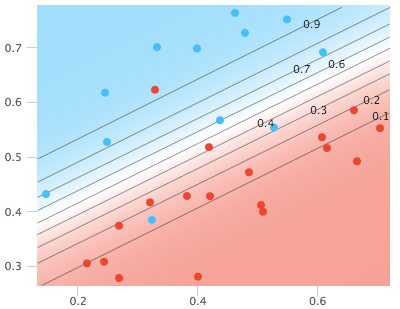
\includegraphics[width=10cm]{slike/logisticna-regresija-konture.png}
\caption{Podatki v prostoru dveh atributov in ločitvena meja med razredi, ki jo uporablja model logistične regresije.}
\label{f:lr-margin}}
\end{figure}

\section{Večrazredna logistična regresija}

Postopek, ki ga bomo tu opisali, se imenuje tudi regresija softmax \angl{softmax regression}\footnote{Pri izpeljavi regresije softmax smo se zgledovali po spletni strani \url{http://ufldl.stanford.edu/tutorial/supervised/SoftmaxRegression/}.}. Nazivi so sicer rahlo zavajajoči, saj gre za klasifikacijsko in ne regresijsko metodo, a po drugi strani čisto informativni, saj v jedru uporabljajo linearno kombinacijo atributov. Za logistično regresijo smo zgoraj omenili, da pretvori atributni vektor $x$ v neko število $f(x)$, tega pa potem v verjetnost ciljnega razreda. Pri večrazredni, tudi imenovani multinomski klasifikaciji, bi lahko izhajali iz predpostavke, da smo za nek atributni vektor za vsakega od razredov izračunali neko število. Recimo, napovedujemo vreme: jasno, oblačno ali deževno. Predstavljajmo si, da imamo nek predpis, ki nam iz dnevne karte Slovenije (vektor atributov) izračuna vektor števil za naš tri razrede. Naj bo ta vektor $z=[2.5, 3.7, 1.9]^T$. Naj nas tu zaenkrat ne bega, kako smo do tega vektorja prišli, a vsekakor opazimo, da to niso verjetnosti. Verjetnosti pa so ravno tiste, ki bi jih od našega napovednega modela želeli. Potrebujemo predpis, funkcijo, ki naš vektor pretvori v verjetnosti, torej predpis, ki stori nekaj z vektorjem $z$ tako, da iz njena izračuna vektor istih dimenzij, kjer so vrednosti verjetnosti razredov, ki se seveda seštejejo v 1. Tak predpis je funkcija softmax:

$$\sigma(z_j) = \frac{e^{z_j}}{\sum_{k=1}^K e^{z_k}}$$

Softmax nam torej naš vektor $z=[2.5, 3.7, 1.9]^T$ pretvori v vektor
$\sigma(z)=[0.21, 0.68, 0.11]$. Funkcija sama poskrbi, da je vektor enotni, saj elemente vektorja ($e^{z_j}$) v funkcijskem predpisu deli z njihovo vsoto, torej jih normira.

V redu. A kako dobimo elemente vektorja $z$? Tako kot pri logistični regresiji, naj bo tudi ta izračunan z linearno kombinacijo atributnih vrednosti. Za $j$-ti razred in vektor atributnih vrednosti $x$ zapišemo torej:

$$ z_j(x)=\theta_{j,0}+\theta_{j,1} x_1 + \ldots + +\theta_{j,n} x_n $$

Z $n$ smo tu označili število atributov. Za bolj kompakten zapis se dogovorimo, kot smo to storili pri logistični regresiji, da uvedemo še $x_0=1$. Vektorski zapis zgornje linearne kombinacije je:

$$ z_j(x) = \Theta_j^T x $$

Naš mutlinomiski logistični model bo torej za primer opisan z vektorjem atributnih vrednosti $x$ vračal vektor verjetnosti, kjer bo posamezen element ustrezal verjetnosti posameznemu razredu:

\begin{equation}
  \nonumber
  h_\Theta(x) =
  \begin{bmatrix}
    p(y=1|x;\Theta_1) \\ p(y=2|x;\Theta_1) \\ \vdots \\ p(y=k|x;\Theta_k)
  \end{bmatrix}
  = \frac{1}{\sum_{j=1}^{k}e^{\Theta_j^T x}}
  \begin{bmatrix}
    e^{\Theta_1^T x} \\ e^{\Theta_2^T x} \\ \vdots \\ e^{\Theta_k^T x}
  \end{bmatrix}
\end{equation}

Za razred $j$ in primer $x$ je torej verjetnost razreda:

$$ p(y=j|x;\Theta_j)=\frac{e^{\Theta_j^T x}}{\sum_{k=1}^K e^{\Theta_k^T x}} $$

Pozor: $\Theta_1$, $\Theta_2$ do $\Theta_k$ so vektorji in parametri modela, posamezen vektor parametrov za posamezen razred. Da bo vse skupaj bolj kompaktno, te parametre lahko združimo v matriko $\Theta$:

\newcommand{\myrule}{\rule[.5ex]{2em}{0.4pt}}

$$
\Theta =
\begin{bmatrix}
  \myrule~\Theta_1^T~\myrule \\ 
  \myrule~\Theta_2^T~\myrule \\
  \vdots \\
  \myrule~\Theta_k^T~\myrule
\end{bmatrix}
$$

Zgoraj smo določili strukturo modela. Model sam pa bo odvisen od vrednosti parametrov modela, torej vrednosti elementov matrike $\Theta$. Te vrednosti moramo določiti tako, da se bo model čim bolje prilegal učnim podatkom, torej podatkom zbranih v matriki atributov $X$ in vektorju razredov $y$. Prileganje moramo opisati kvantitativno, torej določiti cenovno funkcijo $J(\Theta)$. Do te pridemo preko verjetja. Torej, kakšna je verjetnost, da bomo z našim modelom, ki ga določajo parametri $\Theta$, napovedali pravo vrednost razredov:

\begin{equation}
  \begin{split}
    L(\Theta) & = p(y|X;\Theta) \\
    & = \prod_i^m p(y^{(i)}|x^{(i)};\Theta)
  \end{split}
\end{equation}

Verjetje želimo maksimizirati, torej izbrati take parametre $\Theta$, kjer je verjetje največje. Isto enačbo za verjetje smo že videli (poglej poglavje o logistični regresiji). Tudi takrat smo potožili, da je s produkti delati težko in da so vsote bolje. Nič se ne bo spremenilo, če namesto verjetja uporabimo logaritem verjetja:

\begin{equation}
  \begin{split}
    l(\Theta) & = \log L(\Theta) \\
    & = \sum_i^m p(y^{(i)}|x^{(i)};\Theta)
  \end{split}
\end{equation}

Knjižnice z optimizacijskimi funkcijami tipično iščejo minimume. Naša cenovna funkcija bo zato:

\begin{equation}
  \begin{split}
    J(\Theta) & = -l(\Theta) \\
    & = - \log \sum_i^m p(y^{(i)}|x^{(i)};\Theta) \\
    & = \sum_{i=1}^{m} \log\frac{\exp(\theta_{y^{i}}^T x^{(i)})}{\sum_{j=1}^K \exp(\theta^{(j)\top} x^{(i)})} \\
    & = \sum_{i=1}^{m} \sum_{k=1}^{K}  1\left\{y^{(i)} = k\right\} \log \frac{\exp(\theta^{(k)\top} x^{(i)})}{\sum_{j=1}^K \exp(\theta^{(j)\top} x^{(i)})}
  \end{split}
\end{equation}

Zgornja notacija z $\theta_{y^{i}}^T$ je malce čudna, a pomeni, da izberemo tisti $\theta$ vektor, ki ustreza razredu $y^{i}$. To je z vsoto in indikatorsko funkcijo morda še bolj čudno zapisano v naslednji vrstici. Indikatorska funkcija $1\left\{y^{(i)} = k\right\}$ vrne vrednost 1, če je izraz v oklepajo resničen, sicer pa vrednost 0. A je od vseh zapisov prav ta v zadnji vrstici najbolj uporaben. Verjetnosti v imenovalcu moramo tako ali tako izračunati. Shranimo jih v matriki. Potem iz matrike za števec izberemo samo tiste vrednosti, ki dejansko ustrezajo razredu $i$-tega primera.

Kriterijsko funkcijo imamo. Za izračun parametrov modela bomo uporabili gradientni sestop, oziroma katerokoli (boljšo) optimizacijsko metodo, ki pa potrebuje izračun gradienta. Ta je za $k$-ti vektor parametrov, torej za parametre, ki ustrezajo $k$-temu razredu, enak:

\begin{equation}
\nabla_{\Theta_k} J(\Theta) = - \sum_{i=1}^{m}{ \left[ x^{(i)} \left( 1\{ y^{(i)} = k\}  - p(y^{(i)} = k | x^{(i)}; \Theta) \right) \right] }
\end{equation}
%
Poiskati moramo vrednosti parametrov, ki zgornji izraz minimizirajo. Izraz v notranjem oklepaju gre za primere razreda $k$ proti vrednosti 0, če je le ocenjena verjetnost za ta razred visoka (1 minus nekaj, kar gre proti 1, gre skupaj proti 0). Za primere, ki niso v razredu $k$, pa pričakujemo, da je verjetnost tega razreda čim manjša.

Od tu dalje je enostavno. Lahko uberemo metodo gradientnega sestopa in neko začetno matriko $\Theta$ (morda tako, kjer so vse vrednosti enake 0) osvežujemo:

$$ \Theta_k\leftarrow\Theta_k-\alpha\nabla_{\Theta_k} J(\Theta) $$
%
ali pa (bolje) uporabilo postopek kot je L-BFGS iz za to dostopne knjižnice.

\section{Predoločenost}

Model, ki smo ga uvedli zgoraj, je predoločen. Ima preveč parametrov. Rešitev za $\Theta$ je poljubno mnogo. Zakaj? Vzemimo, da vse vektorjem $\Theta_k$ odštejemo nek poljuben vektor $\Psi$:

\begin{equation}
\begin{split}
p(y = k | x ; \theta)
&= \frac{\exp((\theta_k-\psi)^T x)}{\sum_{j=1}^K \exp( (\theta_j-\psi)^T x)}  \\
&= \frac{\exp(\theta_k^T x) \exp(-\psi^T x)}{\sum_{j=1}^K \exp(\theta_j^T x) \exp(-\psi^T x)} \\
&= \frac{\exp(\theta_k^T x)}{\sum_{j=1}^K \exp(\theta_j^T x)}.
\end{split}
\end{equation}

Hm. Torej odštevanje vektorja $\Psi$ ne vpliva prav nič in se iz vseh enačb pokrajša. Torej, lahko vstavimo, da je $\Psi=\Theta_1$ in je potem $\Theta_1-\Psi=0$. Torej, prva vrstica v matriki $\Theta$ ima vse vrednosti nastavljene na nič. In je pri optimizaciji sploh ne rabimo računati. Računamo potem vse ostale vrednosti. Namesto začetnih $k\times(n+1)$ parametrov imamo tako sistem z $(k-1)\times(n+1)$ parametrov. In eno samo rešitev.

\section{Večrazredna in dvorazredna logistična regresija}

Premislimo, kaj je z večrazredno logistično regresijo v posebnem primeru, ko je $K=2$. Naš vektor verjetnosti razredov bo:

\begin{equation}
\begin{split}
h_\Theta(x) & =
\frac{1}{\exp(\Theta_1^T x)  + \exp(\Theta_2^T x ) }
\begin{bmatrix}
\exp( \Theta_1^T x ) \\
\exp( \Theta_2^T x )
\end{bmatrix}
\end{split}
\end{equation}

Ta sistem, kot vemo iz prejšnjega razdelka, je predoločen. Izberemo vektor $\Psi=\Theta_1$ in ga odštejemo od $\Theta_1$ in $\Theta_2$:

\begin{equation}
\begin{split}
h(x) & =
\frac{1}{ \exp( (\theta_1-\theta_2)^T x^{(i)} ) + \exp(\vec{0}^T x) }
\begin{bmatrix}
\exp( (\theta_1-\theta_2)^T x )
\exp( \vec{0}^T x ) \\
\end{bmatrix} \\
& =
\begin{bmatrix}
\frac{1}{ 1 + \exp( (\theta_1-\theta_2)^T x ) } \\
\frac{\exp( (\theta_1-\theta_2)^T x )}{ 1 + \exp( (\theta_1-\theta_2)^T x ) }
\end{bmatrix} \\
& =
\begin{bmatrix}
\frac{1}{ 1  + \exp( (\theta_1-\theta_2)^T x ) } \\
1 - \frac{1}{ 1  + \exp( (\theta_1-\theta_2)^T x ) } \\
\end{bmatrix}
\end{split}
\end{equation}

V zgornji enačbi nadomestimo $\theta_1-\theta_2$ z $\theta$ in dobimo identični model kot pri logistični regresiji. Regresija softmax pri $K=2$ je identična logistični regresiji.

\section{Regularizacija}

Tako, kot se logistična regresija lahko preveč prilagodi učnim podatkom, to velja tudi za mutlinomsko regresijo. Preveliko prilaganje pomeni visoke vrednosti v matriki $\Theta$ (to vemo že iz linearne regresije, pa tudi iz logistične; oboje iz lekcije o polinomski razširitvi učnih primerov). Zdravilo te anomalije je regularizacija. Cenovna funkcija z regularizacijo je:

\begin{equation}
\nabla_{\Theta_k} J(\Theta) = - \sum_{i=1}^{m}{ \left[ x^{(i)} \left( 1\{ y^{(i)} = k\}  - p(y^{(i)} = k | x^{(i)}; \theta) \right) \right] } + \frac{\lambda}{2}\sum_{k=1}^K\sum_{j=1}^n\Theta_{kj}^2
\end{equation}

Gradient se nam skladno z zgornjo spremembo poveča za $\lambda\Theta_k$.

\cleardoublepage
